\documentclass{article}

\usepackage[utf8]{inputenc}
\usepackage[T1]{fontenc}
\usepackage{lipsum}
\usepackage{graphicx}
\usepackage{amsmath}
\usepackage[margin=1in]{geometry}
\usepackage{titlesec}
\usepackage{enumitem}

\titleformat{\section}
{\LARGE\bfseries}{\thesection}{1em}{}

\titleformat{\subsection}
{\Large\bfseries}{\thesection}{1em}{}

\begin{document}
\pagestyle{empty}
\section*{Diagramma di macchina a stati}
\large
\subsection*{Introduzione}
\large
Obiettivi:
\begin{itemize}[label={-}]
    \itemsep0em
    \item Creare diagrammi di stato, come raccordo per la modellazione legata a chart di casi d'uso e classi
\end{itemize}
UML include anche la modellazione di diagrammi di stato, principalmente utilizzati per illustrare \textbf{eventi} e \textbf{transizioni}.\ Un primo approccio a questa nuova tipologia di chart è dedicata mediante una serie di definizioni informali, che possano garantire una corretta visione di quali strumenti siano necessari pur di poter usare questa semantica.\vspace*{14pt}\\
\textit{Definizione informale}\\Un \textbf{evento} è una occorrenza significativa, similmente, anche se ritrae un esempio scontato e banale, può essere (\textit{Alzare la cornetta del telefono}).\vspace*{14pt}\\
\textit{Definizione informale}\\Uno \textbf{stato} è la condizione di un oggetto in un dato momento; riprendendo quanto detto prima potrebbe essere indicato uno stato come segue (\textit{Il telefono non termina di squillare fino a quando il ricevitore non alza la cornetta}).\vspace*{14pt}\\
\textit{Definizione informale}\\Una \textbf{transizione} è la relazione tra due \textit{stati}, la quale indica qualora un \textit{evento} si concretizzi, il \textit{token} si muove dallo \textit{stato iniziale}, o meglio antecedente, verso lo \textit{stato successivo}. Nuovamente, pur di ottenere un caso reale, si può concludere l'esempio aggiungendo (\textit{Quando l'evento di alzare la corntta si realizza, il telefono passa dallo stato sonoro allo stato attivo}).\vspace*{14pt}\\
Tuttavia è bene sin da subito indicare una duplice distinzione dei diagrammi di stato, anche se entrambi sono \textbf{diagrammi comportamentali}, indicata come di seguito:
\begin{itemize}[label={-}]
    \itemsep0em
    \item Un diagramma legato a \textit{behavioral state machine} descrive un \textit{evento comportamentale} del sistema o di una parte del sistema, come un \textbf{attraversamento} dei \textit{vertici} che compongono il chart, connessi mediante \textit{transizioni} 
    \item Un diagramma legato a \textit{protocol state machine} descrive il ciclo di vita oppure sequenze di interazioni valide per parti del sistema. Quindi in questo caso si evince la presenza di un \textit{protocollo}, in grado di poter rescindere quali azioni possano essere considerate corrette o sbagliate
\end{itemize}
Spesso una rappresentazione grafica del diagramma ritrae tutte le entità analizzate, illustrando gli eventi e gli stati di interesse di un oggetto e il comportamento dello stesso in relazione a stimili esterni, quali eventi.\ Rispetto ai modelli osservati fino ad ora, occorre individuare l'atteggiamento differente che avviene mediante gli stati; essi sono utilizzati come participio, per cui in maniera opposta rispetto ad un possibile caso d'uso, il quale esprime esso stesso la partecipazione attiva all'azione, mentre uno stato subisce passivamente l'azione svolta e accettata.\\Le transizioni sono raffigurate come archi, dove al di sopra è posto l'evento, mentre gli stati sono indicativi mediante un rettangolo con i bordi smussati.\vspace*{14pt}\\
\textit{Esempio}
\begin{center}
    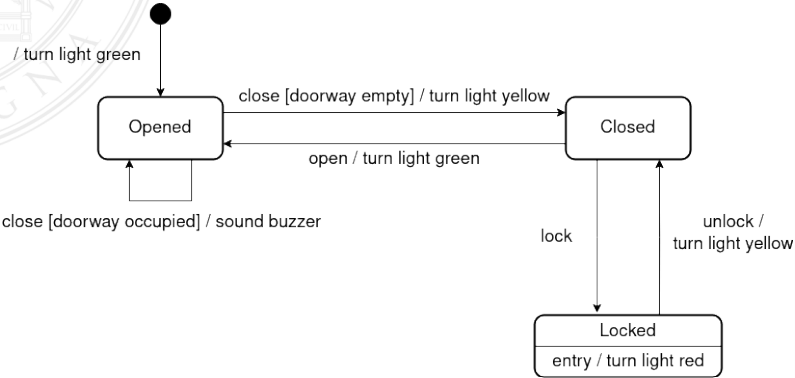
\includegraphics[width=0.8\textwidth]{foto 1.png}
\end{center}
\textit{Nota}: tale modello è usato per esprimere un livello di informazioni piuttosto elevato, molto rigoroso, non contribuendo ad alcuna interpretazione possibile.\vspace*{14pt}\\
Si propone una lettura del diagramma in passaggi consecutivi, che possa anche approcciare a concetti teorici, posta come segue:
\begin{itemize}[label={-}]
    \itemsep0em
    \item Il \textit{nodo totalmente nero} indica il punto di partenza, da cui cominceranno a defluire i differenti token; per certi aspetti simile all'\textit{activities diagram}
    \item Gli stati sono posti dentro rettangoli con bordi smussati. \textit{Opened} rappresenta lo stato iniziale, inoltre si ricorda la denominazione data, un participio, il quale indica un atteggiamento passivo rispetto all'azione corrisposta
    \item Le transizioni consistono nei diversi edge, i quali dallo stato iniziale puntano a quello successivo, ma non è escluso che si verifichi esattamente l'opposto. Effettività, pur sempre rapportate allo stato \textit{Opened} sono \textit{close [doorway occupied]}, la quale indica l'impossibilità nell'apertura della porta, quindi conduce nuovamente allo stesso stato trattato e \textit{close [doorway empty]}, ossia è possibile aprire la porta per poi successivamente chiuderla, ponendo l'evento \textit{close} che varierà lo stato a \textit{Closed} 
    \item Ciò che è posto tra le parentesi quadre, come avviene per \textit{[doorway occupied]}, stabiliscono delle \textit{guardie}, le quali operano in maniera piuttosto selettiva; l'impossibilità che un evento non si verifichi è garantita dalla presenza di tale vincolo, la quale pone un giudizio sulla correttezza del passaggio del token
\end{itemize}
Ultima considerazione aggiuntiva al diagramma prevede che nessuno stato di per sé abbia comportamenti. Uno stato si differenzia da altri corrispettivi poichè prendendo in considerazione \textit{input} differenti corrispondono \textit{output} differenti.
\subsection*{Stato}
\large
Come già ribadito più volte, uno \textbf{stato} è una condizione o situazione durante la vita di un oggetto in cui esso soddisfa una condizione, esegue un'attività oppure aspetta un evento. Riprendendo, uno stato si differenzia dai corrisposti reagendo in maniera totalmente differente rispetto a medesimi input introdotti; tuttavia per essere stabilito tale deve promuovere un medesimo atteggiamento rispetto a stessi dati immessi. Avviene una diversificazione in due successive tipologie, quali:
\begin{itemize}[label={-}]
    \itemsep0em
    \item Stato semplice, non ha vertici interni nemmeno transizioni
    \item Stato composto, contiene una o più sottosequenze, o meglio definiti sotto-stati
\end{itemize}
Inoltre si adotta un'ulteriore distinzione rispetto a possibili comportamenti associati, come segue:
\begin{itemize}[label={-}]
    \itemsep0em
    \item \textit{entry}, è comunicativo qualora siano immesse azioni che stimolino lo stato, per cui producendo un risultato osservabile
    \item \textit{exit} 
    \item \textit{doActivity}, è un behavior eseguito assieme ad ulteriori stati associativi, il quale viene interrotto se non conclude la propria esecuzione qualora si esca dallo stato, a causa della transizione in attivo
\end{itemize}

\subsection*{Transizione}
\large
Una \textbf{transizione} descrive il passaggio \textit{atomico} da uno \textit{stato} ad un corrispettivo, associata in ogni caso ad un \textit{evento}. Le transizioni possono avere delle \textbf{guardie}, le quali pongono la possibilità o impossibilità che si concretizzi un evento e consecutivamente nemmeno la transizione, contrariamente, in assenza, il comportamento interno della transizione dipende totalmente dall'evento posto.\vspace*{14pt}
\begin{center}
    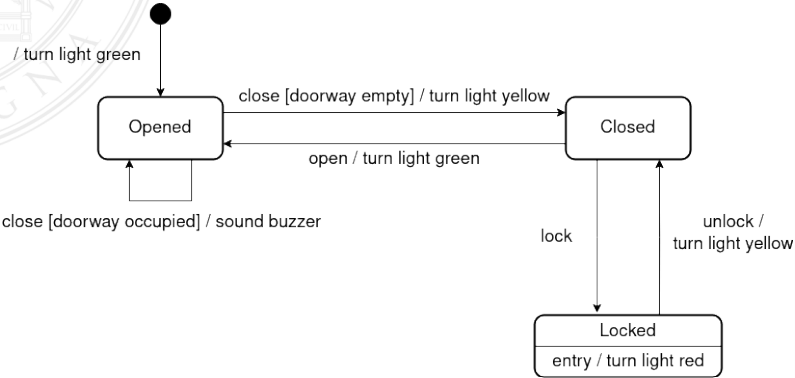
\includegraphics[width=0.5\textwidth]{foto 2.png}
\end{center}

\pagebreak
\end{document}